Un \textit{benchmark} est un test de performance permettant de comparer différentes solutions et outils pour mener à bien un projet.
Pour en réaliser un pour notre projet, il faut prendre en compte plusieurs paramètres. Tout d'abord, nous sommes face à une masse de données très conséquente. Ensuite, il faut aussi prêter attention à ce que les visualisations soient adaptables pour les différents projets utilisant \gls{aikon}. 
Les dernières seront des \textit{preuves de concept}. Il ne sera donc pas possible de les intégrer telles quelles dans l'application. 

Nous allons diviser les solutions envisageables en deux catégories : celles pour visualiser les \textit{regions} au sein du corpus et celles pour analyser les liens de similarités.

\subsection{Visualiser les \textit{regions} au sein du corpus}

Pour réaliser une visualisation des \textit{regions} au sein du corpus, il faut prendre en considération le modèle de données de l'application \gls{aikon}. En effet, il existe plusieurs moyen de rentrer dans le corpus. Il est possible d'accéder aux \textit{regions} par le biais des \textit{witnesses}, des \textit{works}, les \textit{authors} et les \textit{series}. Les données sont également décrites par des métadonnées comme le lieu de conservation, la langue ou le type de document par exemple.


\subsubsection{Zoomable circle packing}

La visualisation en \textit{zoomable circle packing} permet d'entrer dans le corpus par le \textit{witness}. En effet, il n'est pas rare que des manuscrits contiennent plusieurs œuvres. Cette approche est intéressante car elle divise les \textit{regions} selon l'œuvre à laquelle elles sont rattachées. De plus, elle est facilement réalisable en JavaScript avec la bibliothèque \textit{D3.js}. Elle est également simple à comprendre même pour un non-spécialiste. Néanmoins, cette visualisation n'a pas été retenue car il est déjà possible dans l'application \gls{aikon} par le biais du formulaire de recherche à partir de filtres comme le \textit{witness} ou le \textit{work} pour avoir un résultat similaire. 
	
\begin{figure}[H]
	\centering
	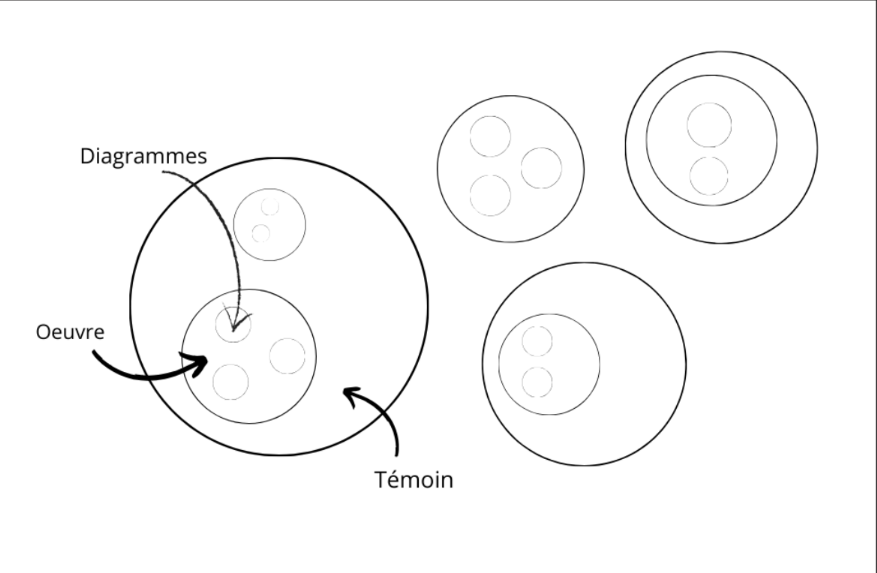
\includegraphics[width=0.8\textwidth]{images/zoomable_circle_packing.png}
	\caption{Maquette de la visualisation en \textit{zoomable circle packing}}
	\label{fig:zoomable}
\end{figure}

\subsubsection{Carte chronologique}

La carte chronologique est une visualisation déjà utilisée par de nombreux projets comme \gls{dishas}. Nous avons élaborer deux versions différentes : 

\begin{itemize}
	\item Une carte sur laquelle sont placés les \textit{authors}, \textit{witnesses} et \textit{works} associée à deux frises chronologiques, une pour filtrer une période donnée comme le Moyen Age et une autre pour définir une période plus restreinte telles que 1250-1350. A l'intérieur de la carte, il est possible d'accéder aux \textit{works}, \textit{authors} et \textit{witnesses}. 
	\item Une carte sur laquelle sont placés les lieux de conservation des \textit{witnesses}. En cliquant sur l'un d'entre eux, tous les \textit{witnesses} présents dedans s'affichent. IL est ensuite possible d'accéder aux \textit{regions} en cliquant sur l'un d'entre eux.
\end{itemize}

Ces deux visualisations ont pour atouts leur faciliter de compréhension (même si la deuxième est plus simple que la première) pour observer la diffusion d'une œuvre dans le temps et l'espace. Néanmoins, elles sont plus complexes à réaliser que la première visualisation car il faut associer une carte et une chronologie. Il est donc nécessaire d'utiliser des bibliothèques JavaScript comme \textit{Leaflet} et \textit{Timeline.js}. De plus, elles n'apportent rien de nouveau à ce qui est déjà possible de faire à partir du formulaire. La visualisation sous forme de carte chronologique peut être intéressante mais face à sa complexité de réalisation, son intégration n'est pas une priorité pour l'application \gls{aikon}. 

\begin{figure}[H]
	\centering
	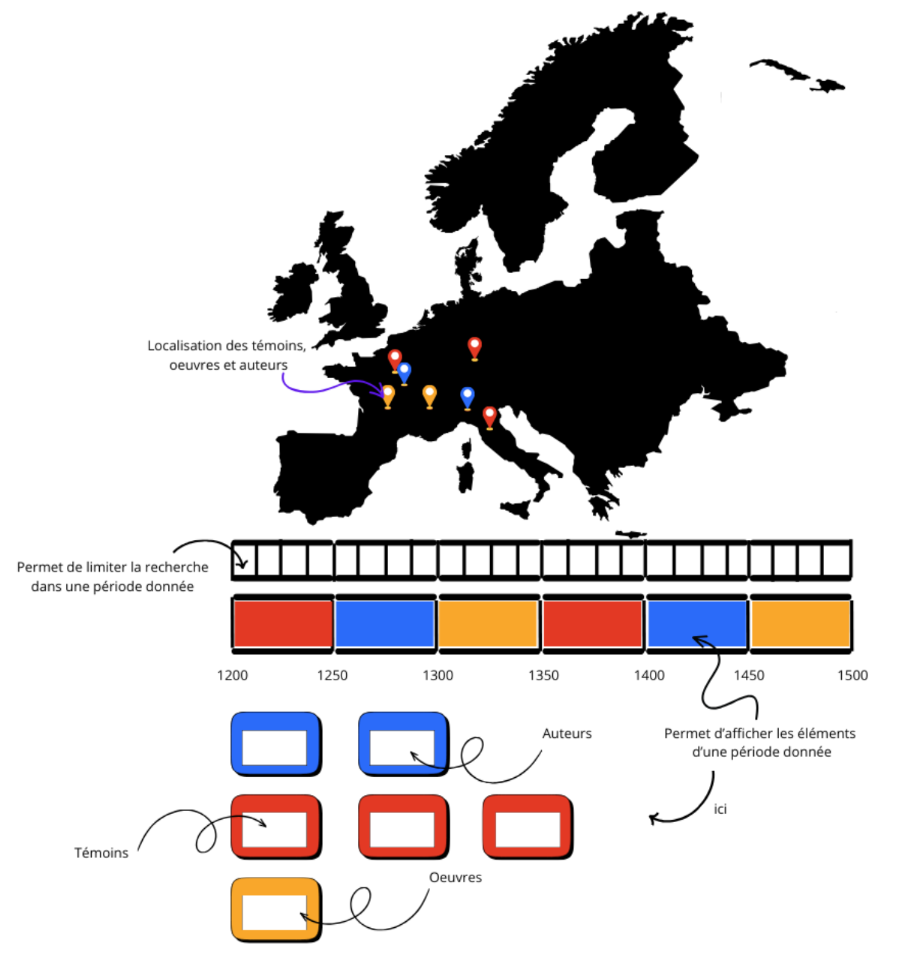
\includegraphics[width=0.7\textwidth]{images/carte_chrono_1.png}
	\caption{Maquette de la première version de la visualisation en carte chronologique}
	\label{fig:chrono1}
\end{figure}

\begin{figure}[H]
	\centering
	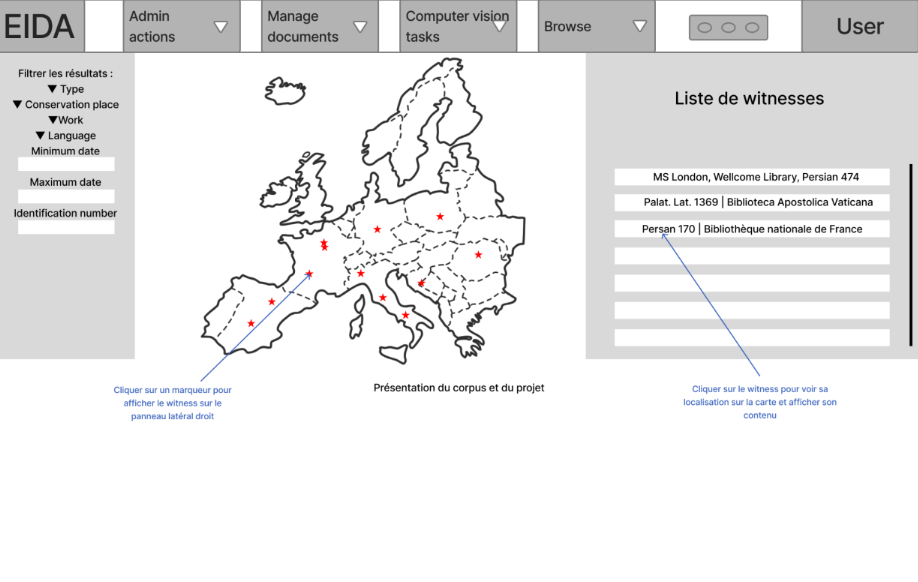
\includegraphics[width=0.8\textwidth]{images/carte_chrono_2.png}
	\caption{Maquette de la seconde version de la visualisation en carte chronologique}
	\label{fig:chrono_2}
\end{figure}


Nous nous sommes rendus compte en imaginant le \textit{benchmark} de ces deux types de visualisation que l'exploration des \textit{regions} au sein du corpus ne constitue pas une priorité pour l'instant. Il est préférable de se concentrer sur le résultat du traitement automatique des similarités. En effet, créer des visualisations pour l'exploration de cet aspect pourrait s'avérer utile pour l'annotation des données mais aussi pour avoir une vue d'ensemble afin de dégager des tendances et des irrégularité dans l'étude de la transmission d'une tradition dans le temps et l'espace. 


\subsection{Visualiser les liens de similarité sous la forme de réseaux}

Pour réaliser une visualisation des \textit{regions} similaires dans l'application \gls{aikon}, il faut isoler deux ou plusieurs \textit{witnesses} à comparer. Il faut ensuite récupérer les données de la table \textit{region-pairs} ainsi que les images des \textit{regions}.
Ensuite, il existe plusieurs formes de visualisation pour représenter les similarités. 


\subsubsection{Hierarchical edge bundling}

La visualisation en \textit{hierarchical edge bundling} permet d'organiser les différentes \textit{regions} en rond et de les relier entre elles par des liens qui se colorent en rouge lorsque nous passons le curseur de la souris dessus. Il est même possible d'organiser les organiser par \textit{witness}. Elle est réalisable en utilisant la bibliothèque JavaScript \textit{D3.js}. Néanmoins, cette visualisation n'a pas été retenue car son organisation en cercle la rend rapidement illisible avec une masse de données trop importante.

\begin{figure}[H]
	\centering
	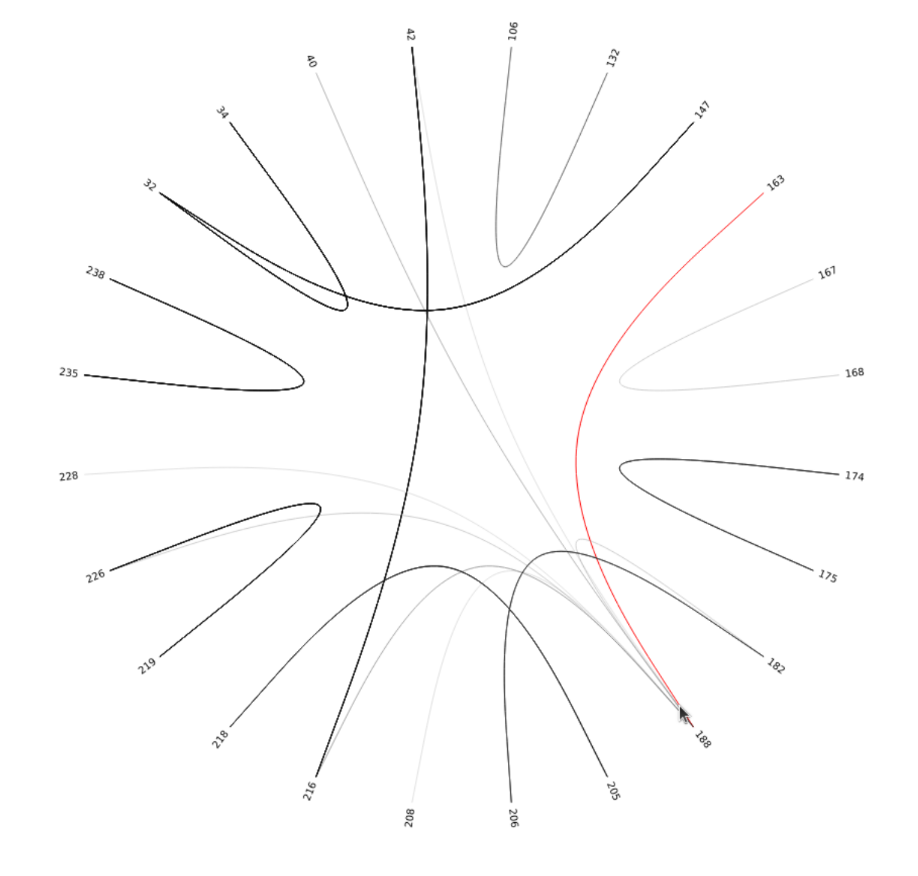
\includegraphics[width=0.5\textwidth]{images/hierarchical_edge_bundling.png}
	\caption{Maquette de la visualisation en \textit{hierarchical edge bundling}}
	\label{fig:hierarchical_edge_bundling}
\end{figure}

\subsubsection{Bipartite graph}

La visualisation en \textit{bipartite graph} est particulièrement efficace tant par sa facilité de compréhension que par sa simplicité de réalisation. Elle permet de représenter les liens entre les \textit{regions} de deux \textit{witnesses} disposées côte à côte. Lorsque nous cliquons sur l'une d'entre elles, tous ses liens avec les autres s'affichent. 

\begin{figure}[H]
	\centering
	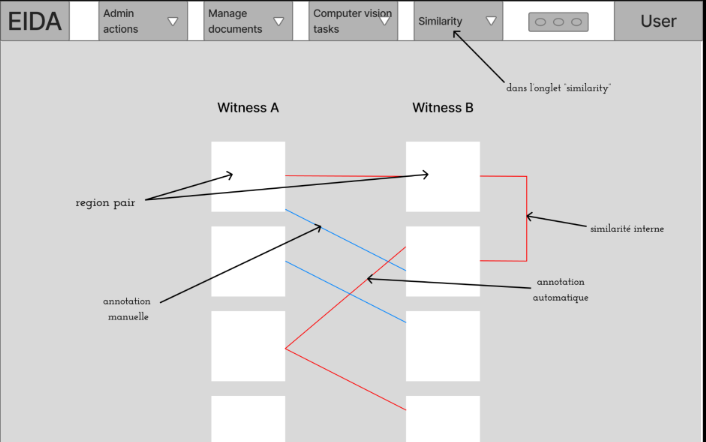
\includegraphics[width=0.8\textwidth]{images/bipartite_graph.png}
	\caption{Maquette de la visualisation en \textit{bipartite graph}}
	\label{fig:bipartite graph}
\end{figure}

\subsubsection{Force-directed layout}

La visualisation en \textit{force-directed layout} permet d'organiser les similarités entre les \textbf{regions} de deux ou plusieurs \textit{witnesses} en réseaux. Son point positif est qu'il permet de donner une vue d'ensemble de toutes les \textit{regions} similaires. 
Ce type de visualisation est réalisable avec des logiciels de création et d'analyse automatique de réseaux.

\begin{figure}[H]
	\centering
	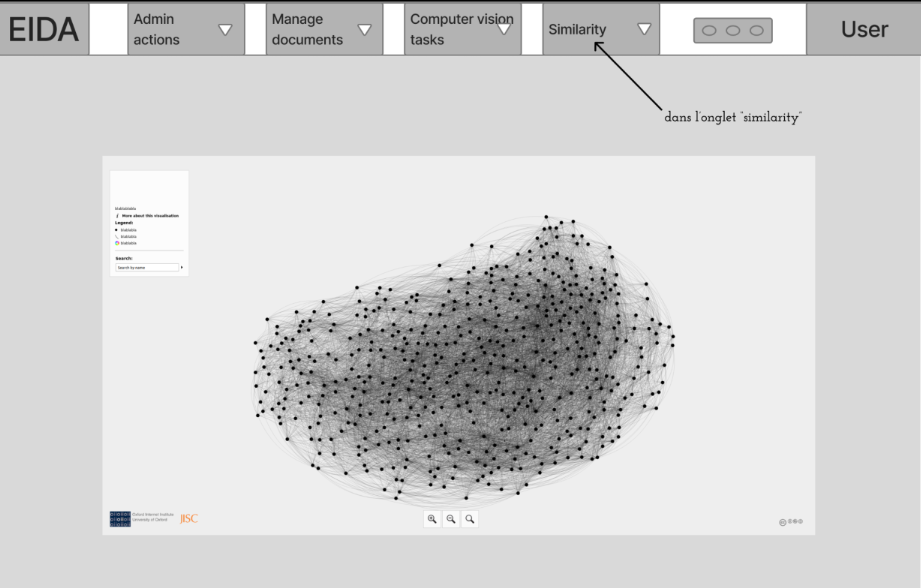
\includegraphics[width=0.8\textwidth]{images/force_directed_layout.png}
	\caption{Maquette de la visualisation en force directed layout}
	\label{fig:force_directed_layout}
\end{figure}

\begin{table}[H]
	\centering 
\begin{tabular}{|p{3cm}|p{5cm}|p{5cm}|}
	\hline 
	Visualisation & Points positifs & Points négatifs \\ \hline
	Zoomable circle packing & Simplicité de compréhension et de réalisation & Possibilité d'avoir un résultat similaire avec le formulaire de recherche \\ \hline 
	Carte chronologique & Facilité de compréhension & Chronophage à réaliser \\ \hline 
	Hierarchical edge bundling & Permet de voir les liens de similarités de toutes les \textit{regions} de plusieurs manuscrits en pouvant les regrouper par \textit{witness} & Devient vite illisible quand il y a une masse de données importante \\ \hline 
	Bipartite graph & Simple à comprendre et à réaliser pour comparer les \textit{regions} de deux \textit{witnesses} & Possibilité de comparer uniquement deux \textit{witnesses}, peut vite devenir illisible et provoquer un arrêt brutal du fonctionnement de l'ordinateur \\ \hline 
	Force-directed layout & Ne nécessite pas de savoir coder car réalisé avec un logiciel et permet d'avoir une vision globale d'un nombre élevé de \textit{witnesses} & Peut vite devenir illisible  \\ \hline 
	\hline
\end{tabular}
\caption{Récapitulatif du \textit{benchmark}}
\label{fig:benchmark_evaluation}
\end{table}

Les deux visualisations les plus adéquates pour notre projet sont le \textit{bipartite graph} et le \textit{force-directed layout}.
